\documentclass[12pt,a4paper]{report}
\usepackage[utf8]{inputenc}
\usepackage[T1]{fontenc}
\usepackage[french]{babel}
\usepackage[french]{nomencl}
\usepackage{lmodern}
\usepackage{graphicx} %Pour les images 
\usepackage{amsmath}
\usepackage{amsfonts}
\usepackage{amssymb}
\usepackage{makeidx}
\usepackage{array} %pour les tableaux \centering pour centrer le tout dans page.
\usepackage{tabularx} %gère automatiqueent la taille du tableau
\usepackage[left=2.5cm,right=2.5cm,top=2.5cm,bottom=2.5cm]{geometry}

%Interligne 1.5
\renewcommand{\baselinestretch}{1.5}

%Pour la page de garde
\newcommand{\hsp}{\hspace{20pt}}
\newcommand{\HRule}{\rule{\linewidth}{0.5mm}}

%HyperRef Conf
\usepackage{hyperref}
\hypersetup{
pdftitle={Mémoire de fin d'étude},
colorlinks=true, %colorise les liens
breaklinks=true, %permet le retour à la ligne dans les liens trop longs
urlcolor=black, %couleur des hyperliens
linkcolor=black, %couleur des liens internes
citecolor=black,    %couleur des liens de citations
bookmarksopen=true,
pdftoolbar=false,
pdfmenubar=false,
}

%Gestion des pied et en-tête de page
\usepackage{fancyhdr}
\pagestyle{fancy}
\lhead{Mémoire de fin d'études}
\chead{}
\rhead{}
\lfoot{Alexis BATTAGLI}
\cfoot{\thepage}
\rfoot{Août 2017}
\renewcommand{\headrulewidth}{0.4pt}
\renewcommand{\footrulewidth}{0.4pt}

%Gestion des titre et indentation
\renewcommand{\thesection}{\arabic{section}}
\setcounter{secnumdepth}{4} % On affiche une numérotation sur une profondeur de 4
\setcounter{tocdepth}{4}        % La table des matières va a une profondeur de 5
% Alignement des titres :
\usepackage{titlesec}
\titlespacing{\chapter} {0pt} {*0} {*0} {}
\titlespacing{\section} {2ex} {*0} {*0} {}
\titlespacing{\subsection} {6ex} {*0} {*0} {}
\titlespacing{\subsubsection} {10ex} {*0} {*0} {}

%Gestion des Acronymes & Glossaire
\usepackage[acronym]{glossaries}
\makenoidxglossaries
\loadglsentries{MyGlossaries.tex}
\loadglsentries{MyAcronymes.tex}

\begin{document}

%Page de garde
\begin{titlepage}
  \begin{center}

    \textsc{\LARGE Mémoire de fin d'étude}\\[2cm]

    \textsc{\Large Ingénieur Informatique\\ spécialité Systèmes et Réseaux}\\[1.5cm]

    % Title
    \HRule \\[0.4cm]
    { \huge Conception et réalisation d'un outil de validation d'équipements CWMP\\[0.4cm] }

    \HRule \\[2cm]
    
\includegraphics[scale=0.2]{./img/imt_mines_ales-bleu.jpg}
    
\includegraphics[scale=0.1]{./img/orange.jpg}
    \\[2cm]

    % Author and supervisor
    \begin{minipage}{0.55\textwidth}
      \begin{flushleft} \large
        \emph{Alternant :} Alexis \textsc{BATTAGLI}\\
        \emph{Maitre d'apprentissage:}Marc \textsc{DOUET}\\
        \emph{Tuteur académique : } Yan \textsc{MORET}
      \end{flushleft}
    \end{minipage}
    \begin{minipage}{0.4\textwidth}
      \begin{flushright} \large
      	\emph{École :} IMT Mines Alès\\
       	\emph{Entreprise :} Orange\\
        \emph{Promotion :} INFRES 7\\
      \end{flushright}
    \end{minipage}

    \vfill

    % Bottom of the page
    {\large Septembre 2014 — Septembre 2017}

  \end{center}
\end{titlepage}

\newpage
\tableofcontents

\newpage
\listoffigures

\newpage
\listoftables

\newpage
\printnoidxglossary[type=\acronymtype]

\newpage
\section*{Remerciments}

\newpage
\section{Introduction}
\subsection{L'entreprise}
\paragraph*{}
Orange est à l’origine une entreprise anglaise de télécommunication. Elle a été rachetée par France Télécom en 2000, entreprise française fondée en 1975, devenant par la suite de ce rachat une société internationale. Au 1er juillet 2013, France Télécom change de nom est devient Orange, société française qui est alors la 121ème entreprise mondiale avec un chiffre d’affaire de 41 milliards d’euros fin 2016. Actuellement, Orange emploie 155 000 personnes mondialement, dont 96 000 en France et possède plus de 263 millions de clients dans le monde répartis dans 29 pays dont 11 pays d’Europe. (Voir carte ci-dessous)
\begin{figure}[!ht]
    \center
    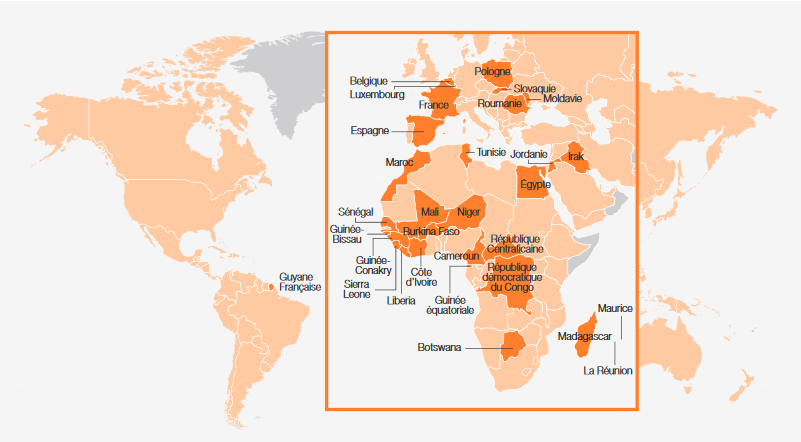
\includegraphics[scale=0.75]{./img/world_orange_2016.PNG}
    \caption{Carte des pays où est présent Orange en 2016}
\end{figure}
\paragraph*{}
Le groupe Orange est majoritairement présent en Europe et Afrique. Il est avant tout un leader de la téléphonie mobile avec un total de 202 millions de clients mobile en 2016 au niveau mondial. Orange est aussi leader dans le domaine de l’accès à Internet avec 18 millions de clients Internet haut débit fin 2016, 265 000 clients \gls{ftth} et 42 millions de clients sur la téléphonie fixe fin 2014 en France. Les pays où le groupe est le plus implanté sont la France, l’Espagne, la Pologne et la Roumanie. Depuis plusieurs années maintenant Orange essaie de se développer également en Afrique dans le domaine de la téléphonie mobile.
\paragraph*{}
Le secteur d’activité principal du groupe Orange reste les Télécommunications, en étant un opérateur téléphonique majeur en France et dans bien d’autres pays tels que la Pologne, l’Espagne, la Roumanie, Côte d’Ivoire, Égypte etc. Orange est également un fournisseur d’accès Internet et depuis quelques années élargit ses activités à la domotique, vente de contenus cinématographique et musical, médical, applications bancaires et automobiles etc.
\paragraph*{}
Les principaux concurrents d'Orange en France dans le domaine \gls{fai} sont principalement Free, Numéricâble, OVH, Nerim, Wifirst et Bouygues Télécoms. Et pour la téléphonie mobile ses principaux concurrents sont SFR, Free et Bouygues Télécom. Tandis qu'au niveau européen sur le domaine téléphonique et \gls{fai}, les principaux concurrents sont Deutsche Telekom, Vodafone et O2 en grande majorité.
\paragraph*{}
La branche où j’effectue mon alternance depuis 3 ans est \gls{ols}. Cette branche concerne tous ce qui touche à la recherche et au développement des produits Orange. Anciennement nommé France Télécom R\&D, puis \gls{olps} en 2007, et enfin rebaptisé \gls{ols} en 2017. Cette branche destinée à la recherche de l’ensemble du groupe Orange emploie 3500 personnes exclusivement en France. Fin 2012, le nombre de brevets déposés par Orange Labs s’élevaient à 7493. La R\&D est très importante pour Orange qui investit chaque année près de 900 millions d’euros dans ce secteur. \\

\subsection{Le contexte}
\subsubsection{Le Device Mangement à Orange}
\paragraph*{}
Mon alternance se déroule plus précisément au sein de l’équipe \gls{care}  qui s’occupe de la gestion des équipements client, c’est-à-dire du « Device Management ».
\paragraph*{}
Le concept de « Device Management » possède plusieurs définitions selon les objets ou équipements gérés, et les équipes qui le mettent en place. Pour nous, le Device Management s'articule autour de quatre axes:
\begin{itemize}
\subparagraph*{}
\item Provsioning: Active ou désactive un service pour le client sur l'équipement adéquate; Applique le bon \gls{firmwareg} selon le service souscrit; Paramètre de manière personnalisé la configuration d'un équipement donné en fonction des services.
\item Assistance: Permet de diagnostiquer à distance un incident sur l'équipement; Déclencher à distance l'exécution d'action permettant de corriger un incident.
\item Tracking: Collecte et stocke des informations sur l'ensemble du parc client.
\item Maintenance: Permet la mise à jour de \gls{firmwareg} à différent temps souhaité.
\end{itemize}
\paragraph*{}
L'architecture du Device Management est découpé en deux zones détaillées comme suis : 
%Import Images
\begin{figure}[!ht]
    \center
    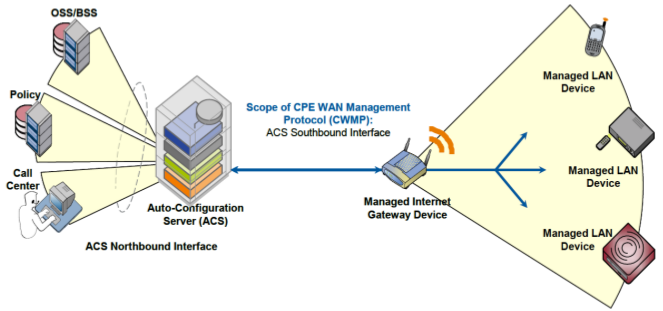
\includegraphics[scale=0.7]{./img/DM-TR-069-screen.png}
    \caption{Réseau de Device Management, côté Opérateur et côté Client}
\end{figure}
\begin{itemize}
\subparagraph*{}
\item Le coté client, où l'on retrouve le réseau privé du client, dit le \gls{lan}, avec généralement divers équipements, que l'on nomme \gls{cpe}, tels que, une passerelle Internet, un décodeur TV, un téléphone, une caméra \gls{ip}, des capteurs domotiques etc.
\item Le coté serveur, se trouvant chez Orange, où l'on va retrouver les serveurs, que l'on nomme \gls{acs}, qui vont permettre de faire ce que l'on nomme du Device Management.
\end{itemize}
\paragraph*{}
L’un des objectifs du Device Management, pour l’équipe \gls{care}, est d’apporter un service d’aide et de dépannage aux clients, tous en restant à distance. Dans le but de ne pas avoir à faire déplacer un technicien sur place, pour un problème qui peut être résolu à distance par l’exécution de scripts, lancement de test et analyse, ou encore correction de bug. Le rôle de l’équipe \gls{care}, est de concevoir l’intégration de ces outils qui pourront être utilisés à distance.
\paragraph*{}
La supervision et la maintenance du parc Orange sont d'autres activités dans le
périmètre de l'activité du Device Management. Ce parc contient les différents produits vendus par Orange et qu’Orange s'engage à maintenir. On comprend alors l'importance des activités de supervision et de maintenance. Pour gérer ce parc, Orange a besoin, entre autres, d'identifier les différents équipements présents et d'accéder à leurs  caractéristiques. Les outils de Device Management  développés au sein de l'équipe \gls{care} permettent, cette fois, de remonter aux \gls{acs} toutes les informations nécessaires pour superviser et maintenir le parc. Il permet également de mettre à jour et corriger des bugs en envoyant de nouvelles versions de \gls{firmwareg} aux équipements concernés. \\
\subsubsection{Document TR-069 et protocole normalisé CWMP}
\paragraph*{} Avant de continuer, il est important de préciser quelques élèments de vocabulaire propre au Device Management et décrire plus en détail comment \gls{acs} et \gls{cpe} communiquent.
\paragraph*{}Comme nous l'avons vu précédemment, un \gls{acs} est un serveur qui permet de manager un \gls{cpe}, et par conséquent de réaliser du Device Management sur le parc client. 
\paragraph*{}Les interactions entre \gls{acs} et \gls{cpe} sont standardisées par le \gls{doctr069g}. Ce document permet, entre autre, de décrire comment implémenter la norme TR-069 sous la forme du protocole \gls{cwmp}, tant sur les \gls{acs} que sur les \gls{cpe}.
\paragraph*{}Ce \gls{doctr069g} est le résultat d'un consortium de plusieurs industriels. Ce consortium, appelé le \gls{bbf}, ce compose de plus d'une centaine de membres dont Orange, CISCO, Deutch Telecom, Huawei, Juniper, le gouvernement du Canada, Intel et bien d'autre. Le \gls{bbf} vise à décrire la gestion des équipements clients, dit \gls{cpe}, par les serveurs de gestion d'équipements, dit \gls{acs}. C'est par le \gls{doctr069g} que le \gls{bbf} décrit un standard permettant la communication entre \gls{cpe} et \gls{acs} pour une bonne gestion des équipements clients.
\paragraph*{}Ce standard décrit un modèle de donnée, que l'on nomme \gls{datamodelg}, comportant une partie commune pour chaque équipement implémentant le \gls{doctr069g}. Le management d'un équipement par un \gls{acs} repose en partie sur la présence de ce \gls{datamodelg}. Le standard décrit également différentes méthodes, que l'on nomme RPC Methode, obligatoire ou facultative, qui doivent être implémentées soit par l'\gls{acs} soit par le \gls{cpe}. Ces RPC Méthodes\footnote{Les principales RPC Methodes des \gls{acs} et \gls{cpe} sont visibles en annexe.} vont permettre la communication entre \gls{acs} et \gls{cpe}, et ainsi rendre possible à l'\gls{acs} le managment de ses \gls{cpe}.
\paragraph*{}Plus précisément, un \gls{cpe}, afin de pouvoir échanger avec un \gls{acs}, doit implémenter le \gls{doctr069g} sous la forme d'un client \gls{cwmp}. Les échanges \gls{cwmp} sont transportés sur du \gls{http} et encapsulés dans des messages \gls{soap}. La création d'une session \gls{cwmp} ce fait toujours par le \gls{cpe}. L'\gls{acs} ne peut pas créer de session, en revanche il possède différentes techniques\footnote{Ces techniques feront l'objet de parties présentées plus loin dans le document.} lui permettant de demander au \gls{cpe} de venir initialiser une session \gls{cwmp}. \\

\subsection{Objectifs}
\paragraph*{}Au cours des trois années passées dans l'équipe \gls{care}, il m'a été confié différents objectifs d'importance et de responsabilité croissante. Ces objectifs m'ont permis de monter en compétences tant sur l'aspect technique que l'aspect transversal du métier d'ingénieur informatique.\\
\subsubsection{Première année}
\paragraph*{}À mon arrivée le principal objectif été de me faire monter en compétence sur le domaine du device management, et plus particulièrement sur le protocole \gls{cwmp}. Il a donc été décidé de me faire tout d'abord monter en compétence sur le côté client, puis sur le côté serveur, par différentes missions que nous verrons par la suite\footnote{La partie intitulée "Monté en compétence sur le protocole \gls{cwmp}" est entièrement dédié à cet apprentissage du domaine du device management et du protocole \gls{cwmp}}. \\
\subsubsection{Deuxième année}
\paragraph*{}En début de deuxième année, ayant acquis les connaissances nécessaires lors de la première année, l'objectif était de me faire développer une application permettant de réaliser une série de test de client \gls{cwmp} de manière automatique\footnote{La partie intitulée "Conception et développement de TINK" est entièrement dédiée à la réalisation de cet outil.}.
\paragraph*{}Un autre objectif de cette deuxième année a été d'encadrer un stagiaire de Master 2 Informatiques, Jean-Pierre ONA, qui devait travailler avec moi sur ce projet. Jean-Pierre a été présent de mars à aout 2016, son sujet de stage portait sur la conception et le développement d'une \gls{ihm} pour l'application de mon projet.
\paragraph*{}Enfin, l'un des objectifs de cette deuxième année était de trouver une personne pour prendre la suite du projet de test d'équipements. Pour ce faire je devais mener une activité de tutorat afin de faire monter en compétence une personne de l'équipe sur ce projet.\\
\subsubsection{Troisième année}
\paragraph*{}Pour la troisième année l'objectif était avant tous de continuer le développement et l'ajout de fonctionnalité à l'application réaliser l'année précédente, mais également de la mettre en production et d'en assurer l'aide aux utilisateurs. 
\paragraph*{}Un autre des objectifs était de prévoir mon départ en réalisant un transfert de compétence sur l'outil développer. Cela devait se faire par la rédaction de différentes documentation permettant aux futurs développeurs de continuer mon travail, ainsi que la présentation de l'outil aux équipes susceptibles de récupérer l'outil.\\


\newpage
\section{Monté en compétence sur le protocole CWMP}
\subsection{Études d'équipements}
\paragraph*{}Ce projet s'est déroulé tous au long de la première année. La personne avec qui je travaillais sur ce projet, Serge MARTIN, étant partie à la retraite en octobre 2015, et ayant dû me consacrer moi-même à d'autre missions, ce projet a été progressivement arrêté durant ma deuxième année. L'un des objectifs de ma deuxième année avait été de continuer ce projet le temps que l'on trouve une autre personne à former pour prendre la suite. Malheureusement, cet objectif n'a été que partiellement réalisé, faute de disponibilité de la part de la personne devant reprendre le projet, menant ainsi à l'arrêt du projet.
\paragraph*{}Le projet consiste à faire différents tests sur des équipements Orange que l’on peut retrouver côté clients. Ces tests peuvent être demandés par d'autres équipes ou bien des membres même de \gls{care}. Ces demandes sont faites lorsque l'ont a besoins de savoir comment fonctionne certains équipements Orange au niveau \gls{cwmp}, connaître leurs comportements réseau dans certaines situations, ou encore récupérer une partie voir l'intégralité de leur \gls{datamodelg}. Le domaine de ces tests est très diversifié et peut prendre quelques heures, comme plusieurs semaines. \\
\subsubsection{Présentation du réseau isolé}
\paragraph*{}Afin de reproduire au mieux les conditions réels, avoir une visibilité intégrale sur les échanges ayant lieu, et un contrôle à tous les niveaux du réseau opérateur, nous avons décidé de reproduire un réseau opérateur que l’on nomme « réseau isolé ». 
\paragraph*{}Ce réseau est constitué d’un micro \gls{dslam} faisant la jonction entre la partie opérateur Orange et les clients Orange. Il permet de gérer les « clients » en leur attribuant une adresse \gls{ip} publique via un service de \gls{dhcp} et en créant des lignes \gls{adsl} avec login et mot de passe attribués. 
\paragraph*{}Du cotés clients, on retrouve les différents types de box internet auxquels sont connectés les équipements clients, dans leur réseau \gls{lan}. 
Du coté opérateur, nous avons mis en place un serveur \gls{dhcp} pour attribuer des adresses \gls{ip} aux machines du réseau opérateur. Un serveur \gls{dns} est également présent pour la résolution des noms. Ce serveur \gls{dns} est aussi utilisé par les box internet des clients comme serveur \gls{dns} primaire. Nous avons aussi deux serveurs \gls{acs}. Un premier du même type que celui utilisé par Orange Labs pour les tests et recherches. Et un second, sous forme de Servlet Java\footnote{La servlet Java fait l'objet d'une sous-partie intitulé "Création d'un \gls{acs} Servlet", puisque j'ai également eu à travailler dessus durant ma première année} qui possède moins de fonctionnalités que le premier, mais qui est très utilisé pour les tests de comportement CWMP\footnote{Les test de comportement font l'objet de la partie intitulé "Test de comportement CWMP d'équipement"}. Vous pouvez voir ci-dessous le plan du réseau isolé que nous utilisons et qui est décrit ci-dessus.
\paragraph*{}
%Import Images
\begin{figure}[!ht]
    \center
    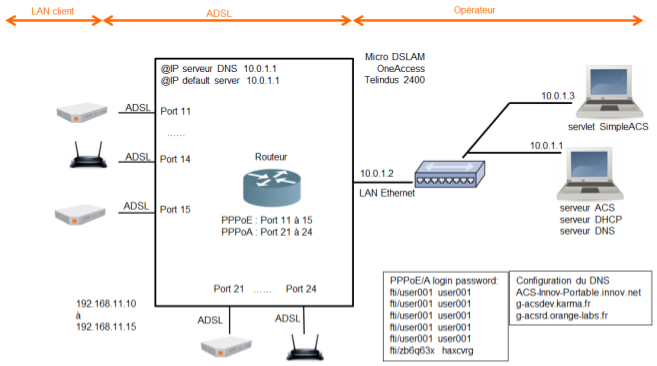
\includegraphics[scale=0.7]{./img/reseau_isole.png}
    \caption{Schéma du réseau isolé}
\end{figure}
\paragraph*{}Nous ne rentrerons pas plus en détail sur ce réseau ici. Il faut également savoir que nous avons placé un concentrateur du côté opérateur, entre les serveurs et le micro \gls{dslam} dans le but de pouvoir analyser le trafic réseau en plaçant un \gls{sniffeurreseaug} tel que Wireshark. 
\paragraph*{}Il arrive parfois que certains équipements dialoguent via \gls{https} avec le serveur \gls{acs}. Ce type de protocole sécurisé nous empêche de faire certains tests liés au protocole \gls{cwmp}, puisque nous n’avons pas les certificats nécessaires au déchiffrage des trames \gls{https}. \\
\subsubsection{Test DNS}
\paragraph*{}Au cours de la première année, une équipe a eu besoin de connaître le comportement des équipements Orange vis-à-vis de leur serveur \gls{dns}. Nous avons donc utilisé le réseau isolé afin de réaliser différents tests sur les équipements en questions.
\paragraph*{}Plus exactement, cette équipe devait migrer des serveurs \gls{acs}. Les \gls{cpe}, selon leur client \gls{cwmp} envoie des requêtes à leur serveur \gls{dns} respectif afin de connaître leur \gls{acs}. Les membres de cette équipe voulaient donc connaître l’impact, en terme de nombre de requêtes \gls{dns}, que cela aller avoir sur les serveurs \gls{dns} des équipements liés à ces serveurs \gls{acs}. Le but premier était de s’assurer que le nombre de requêtes faites par les équipements, pour connaître la nouvelle adresse \gls{ip} de leur \gls{acs}, n’allait pas faire tomber les serveurs \gls{dns} qui sont sollicités par ces équipements. 
\paragraph*{}Nous nous sommes demandés dans un premier temps, quand est ce que doivent apparaître ces requêtes \gls{dns}. Pour ce faire, nous avons regardé ce qui est préconisé par le \gls{doctr069g}, puisqu’en toute logique, les équipements qui communiquent et sont gérés par un serveur \gls{acs}, doivent respecter cette norme le plus fidèlement possible. A partir de la norme, nous avons isolé plusieurs cas d’usage où un équipement se doit de contacter son \gls{acs}, et donc avant cela, faire un appel \gls{dns} pour connaître son adresse \gls{ip}. 
\paragraph*{}Nous avons ensuite mis en place chaque équipement, dans notre réseau isolé, et les avons redirigés vers le serveur \gls{acs} et le serveur \gls{dns} appropriés pour procéder aux tests et à la vérification du respect des cas d’usages. 
\paragraph*{}Il y avait donc deux objectifs. Le premier, était de vérifier si les équipements respectent bien le \gls{doctr069g}. Tandis que le second objectif était de contrôler et relever le nombre de requêtes faites par les équipements vers leur serveur \gls{dns}. 
\paragraph*{}Après avoir testé les différents cas d’usage, sur tous les équipements, il apparaît que certains équipements ne respectent pas le \gls{doctr069g} en termes d'appel \gls{dns}. Certains cas d’usage sont tous simplement ignorés par l'équipement, ce qui représente une grave
erreur d'implémentation du \gls{doctr069g} sur ces équipements. Afin que ces erreurs soient corrigées, nous avons remonté ces anomalies au service qui veille au respect du \gls{doctr069g} et qui font les correctifs des bugs sur les équipements. Nous avons également pu donner des éléments de réponse à la première question par le biais d’un rapport des tests effectués et de présentations aux cours de réunions d'avancement. Au vu des données que nous leur avons remonté, ils ont pu déduire que l'impact du nombre de requête envoyées aux serveurs \gls{dns} ne générerait pas une surcharge des serveurs. \\
\subsubsection{Test de comportement CWMP d'équipement}
\paragraph*{}Les tests CWMP sont des tests qui nous sont demandés par notre équipe de manière irrégulière selon les besoins de l'équipe. Dans l’équipe nous utilisons, aux cours de projet, de nombreux équipements Orange. Le but de ces tests est de connaître les caractéristiques \gls{cwmp} de ces équipements que nous utilisons. Mais aussi être capables de savoir comment ils réagissent dans différentes situations et savoir comment leur client \gls{cwmp} implémente le \gls{doctr069g}. Bien entendu, nous ne testons ici que des équipements embarquant un client \gls{cwmp} capable de communiquer avec son \gls{acs}.
\paragraph*{}A chaque fois que l’équipe récupère un nouveau device susceptible de pouvoir faire du Device Mangement, il doit faire l’objet de ces tests \gls{cwmp}. L’ensemble des résultats de ces tests sont ensuite documentés et archivés afin de pouvoir être réutilisés si besoins. Ces demandes peuvent permettre d'anticiper la venu de nouveaux équipements dans le parc client d'Orange, elles permettent de savoir si nous auront des difficultés à manager ces nouveaux équipements avec la version actuelle de Karma. 
\paragraph*{}Le \gls{doctr069g} est extrêmement long et décrit l'ensemble des régles qu’un \gls{cpe} ce doit d'implémenter, avec plus ou moins de rigueur dans certain cas. Pour tester les équipements que nous recevons, il a été décidé de regarder le respect de 4 points qui sont les plus importants pour les travaux fait dans l’équipe. Ces 4 points\footnote{Nous ne rentrerons pas dans le détail technique de ces quatre tests} ont été sélectionné pour être testé systématiquement car ce sont ceux qui sont le plus souvent demandé par les membres de l’équipe. Un cinquième point a été rajouté récemment avec la création et l’ajout dans le réseau isolé de l’ACSServlet\footnote{Voir la partie intitulé "Création d'un ACS Servlet"}. Ce cinquième test que j’ai pu rajouter consiste à extraire l’intégralité du {datamodelg} d’un équipement. L’extraction du {datamodelg} d’un équipement fait souvent l’objet de demande externe, et fait appel à des fonctionnalités \gls{cwmp} qui sont intéressantes à être testées pour chaque équipement.
\paragraph*{}Pour procéder aux tests, il faut avant tout pouvoir placer les équipements dans notre réseau isolé, ce qui nécessite parfois son amélioration. Les améliorations et modifications peuvent être faites à plusieurs niveaux. Cela peut être une modification de la configuration du micro \gls{dslam}, ajouter de nouveaux types de connections\footnote{Les équipements que nous avons peuvent communiquer soit par PPPoE soit par PPPoA, cela nécessite la configuration de port dédiés à ces deux types de connections.} au micro \gls{dslam}, rajouter des plages d’adresses sur le serveur \gls{dhcp}, ou bien encore créer de nouveaux domaines dans la configuration du serveur \gls{dns}.
\paragraph*{}Cependant, il arrive que l’ajout de l’équipement dans notre réseau isolé ne soit pas possible. Soit à cause de critère physique, comme on a pu le rencontrer avec des dispositifs 4G Huawei, auquel cas nous ne pouvons pas procéder à certains tests, voir à l’intégralité des tests. Soit, à cause de contraintes techniques, qui nous empêche de pouvoir faire le moindre test. Cela arrive lorsque l’équipement utilise un certificat \gls{ssl}, que nous ne possédons pas, dans ce cas aucuns des tests ne sont possibles.
\paragraph*{}De manière générale, les 4 principaux tests sont faits à partir de scripts JavaScript exécutés depuis le serveur \gls{acs}\footnote{C'est ce serveur même qui est utilisé pour la recherche et l'anticipation.} vers lequel remonte les équipements dans le réseau isolé. Tant dit que le cinquième test est fait en redirigeant l’équipement vers l’ACSServlet. Lorsque nous rencontrons un problème avec un équipement, empêchant son installation dans le réseau isolé, nous faisons les tests sur le réseau public. Mais cela rend les tests plus longs et compliqués. Il faut parfois trouver de nouvelles façons de faire et cela ne suffit pas toujours rendant parfois des tests impossibles. \\
\paragraph*{}Ce projet s'est déroulé lors de ma première année. L'étude d'équipements aussi bien comportement \gls{cwmp} que \gls{dns}, la mise en place du réseau isolé et la restitution sous forme oral et écrite des rapports de test, m'auront permis d'acquérir de solides bases sur le protocole \gls{cwmp}, et une excellente entrée en matière dans le Device Management. Cela m'aura également permis de renforcer mes compétences en Système et Réseaux, particulièrement sur la configuration de serveur \gls{dns} et \gls{dhcp} Mais aussi dans tous ce qui est protocole de communication et gestion d'OS. Enfin, cela m'aura permis de renforcer mes compétences en rédaction et présentation oral.\\
\subsection{Étude de client CWMP}
\paragraph*{}Afin de rentrer plus en profondeur sur les spécificités d'implémentation du \gls{doctr069g} pour un \gls{cpe}, j'ai étudié lors de ma première année deux clients \gls{cwmp}. L'étude de ces clients \gls{cwmp} avait pour objectif de détermine quel pouvait être les clients susceptible d'être réutiliser par des équipements du parc Orange, afin de faciliter leur management par Karma. \\
\subsubsection{Client EasyCWMP}
\paragraph*{}L’objectif était de voir dans un premier temps si dans le domaine de l’open source il existe des clients \gls{cwmp} qui ont été développé. Puis, après avoir listé les différents clients \gls{cwmp} open source, je devais récupérer et tester ceux qui semblaient les plus prometteurs et qui implémentent le plus fidèlement le \gls{doctr069g}.
\paragraph*{}Afin de correctement comparer les différents clients open source, et vérifier qu’ils respectaient bien le \gls{doctr069g}, j’ai lu l’intégralité du \gls{doctr069g} écrite par le \gls{bbf}. Cela m’a permis de monter rapidement en compétence sur le sujet. De plus, la norme étant rédigée en anglais cela m’a également permis de monter en compétence sur l'anglais techniques.
\paragraph*{}La comparaison entre les clients open source trouvés ne sait pas faite uniquement sur le respect de l'implémentation du \gls{doctr069g}. Le logiciel devait être régulièrement tenu à jour, et le projet open source devait être encore "vivant", c'est à dire que la communauté derrière le développement du client devait être active. Il donc fallu s'intéresser plus en détail sur la provenance des clients, vérifier qu'une documentation était présente et à jour, ainsi que regarder la date des dernière version des clients sélectionné.
\paragraph*{}A la suite de cette comparaison théorique des différents clients \gls{cwmp} que j’ai pu identifier, il a été décidé de n’en récupérer qu’un seul, nommer EasyCWMP et développer en C par l’entreprise PIVA Software. Seul le code source est disponible sur leur site. Les documentations d’installation et de spécifications n’étaient pas accessibles librement. Pour les récupérer il faut les commander, et donc les payer à PIVA Software, mais nous n'avons pas juger cela comme étant un frein.
\paragraph*{}Nous nous sommes intéressés à ce client \gls{cwmp} open source car il est le seul à implémenter toutes les méthodes obligatoires du \gls{doctr069g}, contrairement aux autres clients open source rencontrés qui ne les implémentes jamais toutes. De plus, nous avons pu voir qu’il était très régulièrement mis à jour. Bien entendu cela était purement théorique à ce moment puisque nous n'avions pas encore pu tester le client en question.
\paragraph*{}Après avoir récupéré le code du logiciel, l’objectif était de l’installer sur un PC afin de le faire remonter vers l'\gls{acs} utilisé pour la recherche et l'anticipaition, que l'on nomme g-acsdev. 
\paragraph*{}L’une des difficultés a été de l’installer sans avoir de documentation, d’autant plus que c’était la première fois que je devais réaliser ce type d’installation en compilant le programme et en installant toutes les libraires dépendantes entre elles. Cela m’a permis de monter en compétence en C puisque je devais comprendre comment compiler le client en C avec ses différentes librairies. Puis comprendre comment, lancer le client, modifier sa configuration, utiliser les différentes méthodes \gls{cwmp} qu’il implémente pour vérifier leurs bon fonctionnement, et enfin le faire communiquer avec g-acsdev. Toutes ces étapes de compilation, configuration et test, ce sont faites sur une machine linux. Une partie du code du client était en Shell, ce qui m’a permis de monter en compétence en Unix également. Mon tuteur m’a expliqué de nombreux aspects de C et de Shell afin de comprendre au mieux le code du client.
\paragraph*{}Après avoir réussi à faire communiquer parfaitement le client EasyCWMP avec g-acsdev et avoir testé les méthodes \gls{cwmp} qu’il implémente, il m’a été demandé de modifier le code du client. L’objectif était de rajouter des paramètres dans son \gls{datamodelg} et de voir ces modifications apparaitre dans l’interface web de g-acsdev lorsque l'on explorerai son \gls{datamodelg}. Cela m’a permis de rentrer plus en détail dans le code du client, puisque rajouter des branches au \gls{datamodelg} implique de modifier le code du client à différents niveaux. Tant au niveau C que Shell, j’ai dû comprendre comment le logiciel était codé, la relation entre les différents fichiers et appels de librairie. Ce qui m’a également permit de monter de nouveau en compétence en C mais également d’apprendre à comprendre un code que l’on récupère, le tout sans aucune documentation.
\paragraph*{}Cette activité m’aura donc apporté énormément dans plusieurs domaines techniques tels que le C, le Shell et renforcer ma monter en compétence sur le protocole \gls{cwmp}. Elle m’aura également permis de voir comment se déroule une activité de bout en bout de manière totalement autonome. A la fin de l’activité il m’a également était demandé de créer une documentation sur l’installation des différents prérequis et du client EasyCWMP même, ce qui m’a permis d’apprendre à rédiger une documentation. De plus, le fait d’avoir fait des recherches dans le domaine de l’open source, m’a aidé à mieux comprendre l’open source avec ces différentes normes et licences, les projets collaboratifs etc. Enfin, cette activité m’aura permis de véritablement rentrer dans le device management et de mieux comprendre le côté client. \\
\subsubsection{Comparaison EasyCWMP et tr69agent}
\paragraph*{}Actuellement tous les constructeurs d’équipement n’implémentent pas
systématiquement un client \gls{cwmp} sur leurs équipements. Cela rend impossible le device management lorsqu’un client achète un équipement chez un de ces constructeurs. Or, Orange s’engage à pouvoir manager l’ensemble des équipements connectés à la LiveBox du client. Par conséquent, nous avons décidé de fournir ce que l’on appelle un « toolkit \gls{cwmp} », qui aurait pour but d’aider les constructeurs qui le souhaitent, à implémenter sur leurs équipements un client \gls{cwmp}. Ce client serait certifié par Orange comme étant capable de communiquer avec nos serveurs \gls{acs}, et donc être manager. La question qui s’est donc posé, était de savoir ce que contiendrait le toolkit proposé par Orange.
\paragraph*{}Nous avons dégagé quatre propositions de contenu du toolkit. Ces quatre propositions de contenue du toolkit ne pourront pas être décrites ici. Afin de départager ces différentes possibilités de contenu nous devions apporter des éléments de comparaison. Par ailleurs, ce n’est pas nous qui avons rendu la décision final, mais les responsables de HomeService\footnote{HomeService correspond au service en-dessous d'\gls{ols}.} qui à partir de cette étude ont pu rendre une décision sur la stratégie à adopter.
\paragraph*{}Ces propositions ont amené à comparer le client EasyCWMP au client nommé tr69agent. Ce client \gls{cwmp} a été développé par Orange. Bien que nous possédions l’intégralité de la documentation et des droits liés à ce logiciel, nous devions vérifier s’il était plus avantageux que le client proposé par PIVA Software. Mon rôle dans cette étude a donc été de comparer ces deux clients et ainsi déterminer quels sont les points faibles et points forts de chacun de ces deux clients.
\paragraph*{}Pour ce faire je leur ai fait passer les tests de comportement \gls{cwmp} et tests \gls{dns}. Les deux clients ont été installés dans des environnements identiques afin de ne pas perturber les résultats. L’analyse de ces tests n’a pas permis de départager les deux clients. En revanches, aucun des deux ne les satisfaisaient complétement, ce qui impliquait que peu import le client qui serait choisi, il faudrait le retravailler afin de le rendre parfaitement en adéquation avec le \gls{doctr069g}.
\paragraph*{} Je suis donc rentré plus en détails dans la comparaison, et j’ai regardé du côté de leurs caractéristiques. Tels que, le poids du logiciel après installation, le langage de programmation utilisé, la clarté de leur code, et les méthodes \gls{cwmp} obligatoires et facultatives implémentées.
\paragraph*{}En dehors de cet aspect technique de comparaison des deux clients, j’ai pu voir comment mener une étude, présenter des résultats et préparer leurs présentations. De plus, j’ai rédigé un rapport sur l’ensemble des tests de comparaison des deux clients, ce qui m’a permis de m’exercer sur l’aspect rédactionnel. Je n’ai malheureusement pas pu assister à la présentation finale puisque cela s’est produit lors de l’une de mes périodes de cours, mais j'ai pu participer à la préparation de la présentation et du support. \\
\subsubsection{Résultats} %conséquence : lancement du projet toolkit !
\paragraph*{}À la suite de la comparaison entre les client \gls{cwmp} EasyCWMP et tr69agent, une des quatre propositions a été retenu. Cette solution consiste, entre autre, à fournir au sein du toolkit le client tr69agent, une documentation permettant l'intégration du client, ainsi qu'une plateforme de test\footnote{La réalisation de cette plateforme fait l'objet de la partie suivante, intitulé "Conception et développement de TINK"} d'implémentation de client \gls{cwmp}. 
\paragraph*{}Les études de ces deux clients m'auront permis de renforcer mes compétences sur le protocole \gls{cwmp}, en particulier sur le côté client. Mes compétences rédactionelles auront également été renforcé. \\
\subsection{Création d'un ACS Servlet}
\paragraph*{}Après être monté en compétence sur \gls{cwmp} et avoir travaillé du côté client du device management avec EasyCWMP et tr69agent, j’ai travaillé du côté serveur. Ce projet s'inscrit encore une fois dans le courant de ma première année.
\paragraph*{}Dans le cadre des tests d'équipements, nous avions besoin d’un deuxième \gls{acs} dans le réseau isolé afin d’effectuer certain tests. C’est pourquoi, un des membres de l’équipe a conçu ce que l’on appelle une \gls{servletg}. Cette \gls{servletg} est codée en langage Java, et se comporte au sein du réseau isolé comme un serveur \gls{acs}. La \gls{servletg} s’installe sur un serveur web installé sur un PC du réseau isolé, permettant ainsi d’avoir un équivalent de serveur \gls{acs} mais extrêmement minimalisé.
\paragraph*{}L’avantage d’avoir une servlet comme \gls{acs} est que l’on peut y rajouter les fonctionnalités dont nous avons besoin. Elle est également facile à installer, puisqu’il suffit uniquement d’un serveur web.
\paragraph*{}On m’a donc demandé de reprendre la \gls{servletg} déjà faite et de l’améliorer afin que dans un premier temps elle puisse extraire le \gls{datamodelg} d’un équipement qui viendrait dialoguer avec elle. Par conséquent, elle devait aussi pouvoir communiquer avec un maximum d'équipements qui implémentent le \gls{doctr069g}. A l’origine, la \gls{servletg} qui a été développé ne pouvait communiquer qu’avec un nombre restreint de types d'équipements à cause de contraintes techniques que je devais donc résoudre.
\paragraph*{}
%Import Images
\begin{figure}[!ht]
    \center
    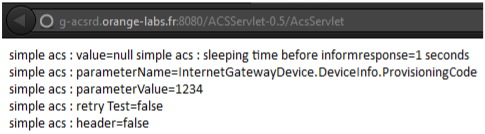
\includegraphics[scale=0.9]{./img/acs_servlet_05.png}
    \caption{Affichage web de l’ACSServlet-0.5, ancienne version}
\end{figure}
\paragraph*{}Comme on peut le voir ci-dessus, la dernière version de la \gls{servletg}, nommé « ACSServlet-0.5 » était extrêmement minimaliste en termes d'affichage. L'état des paramètres utilisés pour les tests d'équipements était modifié via l’url et aucune vérification n’était faite sur la cohérence des valeurs entrées. Par ailleurs, elle implémentait un nombre limité de méthodes \gls{cwmp}. Je devais donc améliorer l’interface web afin de proposer une solution plus simple pour modifier les paramètres. De plus, j’ai pensé qu’un contrôle des valeurs de ces paramètres serait un plus et une sécurité pour l’utilisateur. Le tous devait bien entendu pouvoir fonctionner avec le plus grand nombre de device possible en implémentant davantage de méthodes \gls{cwmp}. Enfin, elle devait pouvoir extraire systématiquement le data model de l’équipement dans un fichier au format .csv.
\paragraph*{}Comme pour les précédentes activités, j’étais libre de procéder dans l’ordre que je souhaitais pour réaliser ce travail. L’objectif étant là encore de me faire gérer de bout en bout une activité, découper les différentes tâches et étapes, le tout sans hésiter à aller voir les personnes susceptibles de m’apporter des informations et explications dans les domaines dont j’avais besoin.
\paragraph*{}J’ai tout d’abord cherché à comprendre le code de la \gls{servletg} que l’on m’avait donné. N’ayant pas vraiment de connaissance dans le langage Java, je devais également monter en compétence dans ce domaine. Cela m’a pris plusieurs jours pour voir et comprendre le code, les fonctionnalités mises en place, ainsi que les outils utilisés pour développer la \gls{servletg}.
\paragraph*{}Je me suis familiarisé avec le code en ajoutant des méthodes \gls{cwmp} qu’un serveur \gls{acs} doit avoir pour communiquer avec différents équipements. J’ai pu identifier et implémenter ces différentes méthodes depuis le \gls{doctr069g}, mais également en analysant les échanges de trames sur le réseau isolé entre un équipement et son \gls{acs}. L’implémentation de ces méthodes m’a permis de me familiariser plus rapidement avec l’ensemble du code. J’ai également pu avoir plusieurs explications de la personne qui a développé les premières versions de la \gls{servletg}.
\paragraph*{}Une fois cette première étape de découverte passée, j’ai pu faire communiquer la \gls{servletg}, avec ces nouvelles méthodes, au client EasyCWMP sur lequel j’avais travaillé précédemment. Et ainsi vérifier son bon fonctionnement sur un premier type d’équipement.
\paragraph*{}J’ai part la suite réfléchie à la méthode à employer pour réaliser l’extraction du \gls{datamodelg} d’un équipement quelconque. Un \gls{datamodelg} ce présentant sous forme d’un arbre. Je me suis donc renseigné sur les différents types de parcours d’arbre possible et algorithme associé, afin de choisir le plus optimisé, mais aussi le plus en adéquation avec les contraintes techniques que j’avais. Le \gls{datamodelg} devait être extrait sous forme d’un fichier .csv.
\paragraph*{} Une fois l’implémentation de cet algorithme fait, j’ai cherché à le tester sur un maximum d’équipements. Il fallait donc modifier la \gls{servletg} de telle façon à ce qu’elle puisse s’adapter à l’équipement qu’on lui présente en entrée, et communiquée avec. Cela a été assez compliqué et partiellement réaliser, puisque tous les équipements ne dialogue pas forcément de la même façon, et apporte donc régulièrement de nouvelles contraintes. Ce travail d’adaptation de la \gls{servletg} à un équipement nécessiterait beaucoup plus de temps que celui disponible pour l’activité entière.
\paragraph*{}Après avoir permis à la \gls{servletg} de communiquer avec différents équipements et d’extraire leur \gls{datamodelg}, j’ai voulu faire des tests d’extraction de \gls{datamodelg}. L’objectif était de comparer le temps d’extraction du \gls{datamodelg} de plusieurs équipements depuis ma \gls{servletg}, avec le temps d’extraction depuis un script JavaScript exécuté sur le serveur \gls{acs} g-acsrd. Ces mesures ont été réalisé selon différents critères tels que, le nombre de paramètres (feuille), le nombre de groupe de paramètre (branche), le poids final du \gls{datamodelg} dans un .csv et l’équipement dont le \gls{datamodelg} est extrait \footnote{Les capacités de RAM et cpu de l'équipement sont très influentes sur l'éxecution des requêtes permettant de parcourir le \gls{datamodelg}}. Cela m’a amené à optimiser mon algorithme d’extractions, et plus généralement le code entier de ma \gls{servletg}.
\paragraph*{}Une fois l’étape d’optimisation du code effectué, j’ai créé une page d’accueil de la \gls{servletg} en html et css avec un formulaire pour modifier les paramètres plus proprement. De plus, lors de l’envoie des valeurs des paramètres, j’ai rajouté une vérification afin de détecter différentes anomalies ou valeurs impossibles qui serait entré par l’utilisateur et entrainerais un blocage de l’équipement.
\paragraph*{}Enfin, après avoir testé le bon fonctionnement de la \gls{servletg}, j’ai pu l’installé sur le serveur g-acsrd et donc la rendre accessible depuis l’extérieur, comme on peut le voir ci-dessous.
\paragraph*{}
%Import Images
\begin{figure}[!ht]
    \center
    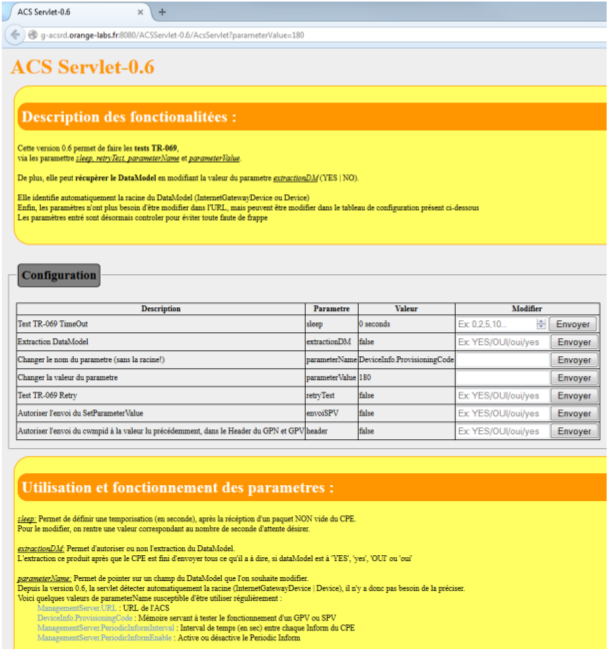
\includegraphics[scale=0.74]{./img/acs_servlet_06.png}
    \caption{Affichage web de l’ACSServlet-0.6, nouvelle version}
\end{figure}
\newpage
\paragraph*{}J’ai également ajouté une partie sur la page d'accueil expliquant les fonctionnalités et le rôle de cette \gls{servletg}, avec des exemples de valeurs attendues pour les paramètres et une note d'explication pour chacun d’eux.
\paragraph*{}Cette activité m’aura permis de monter en compétence en Java, plus particulièrement du côté \gls{servletg}. Mais également de m’améliorer dans la gestion d’une activité de plusieurs mois entre coupé par les périodes de cours et les autres activités. Enfin, j’ai pu de nouveau monter en compétence sur \gls{cwmp}. \\
\subsection{Impact sur mon parcours}
\paragraph*{}Comme nous avons pu le voir tous au long de cette partie, les activités réalisées durant la première année de mon alternance m'ont permis de monter rapidement en compétence sur le protocole \{cwmp], et permis d'avoir une bonne vision du domaine du device management. La lecture du \gls{doctr069g}, puis l'activité de test d'équipements réalisé sur l'ensemble de l'année, m'ont permis de comprendre le protocole \gls{cwmp}, voir différentes implémentation et comportement d'équipements. Le projet d'étude du client EasyCWMP, puis la comparaison avec le client tr69agent, m'ont permis de rentrer plus en profondeur sur les aspects clients du protocole, mais aussi de développer des compétence en développement et génie logiciel. Enfin, le projet d'ACS Servlet, m'a quant à lui permis de rentrer plus en détails sur l'implémentation de la partie serveur du protocole. J'ai par ailleurs pu travailler avec une grande partie des membres de mon équipe durant ces différents projets, me permettant ainsi de m'intégrer au mieux au sein de mon service et de mon entreprise. 
\paragraph*{}Sur les domaines techniques, j'ai pu renforcer mes compétences en administration réseaux et système développer durant mon DUT R\&T. Plus précisément, j'ai renforcé mes compétences sur la configuration de serveur \gls{dns} et \gls{dhcp} lors des études de comportement de client. J'ai pu également acquérir des bases de développement en C et Java dont je n'avais que très peu de notion avant mon arrivé. Ces bases en développement, comme nous le verrons par la suite, ont été extrêmement utile et sollicité durant la suite de mon alternance. De plus, mes compétences acquises en entreprise sur le domaine logiciel, ont pu être renforcées par les cours de développement et le projet Java de première année suivi à l'école. 
\paragraph*{}Sur les domaines transversales, j'ai pu acquérir de solide base en rédaction de documentation et rappport d'étude. Ces documents ont été rédigé en français, mais cela m'a permis d'avoir connaissance du rendu attendu pour ces différents type de document. J'ai également pu acquérir, grâce au projet de test d'équipements, des compétences sur les aspects de travail collaboratif. Enfin, le fait d'avoir eu une très grande autonomie dans sur l'ensemble des projets m'a permis de renforcer mes compétences en gestion du temps, planification et organisation de projet. Là encore, ces compétences seront grandement sollicitées et renforcées par la suite.
\paragraph*{}Ainsi, ces projets n'auront pas uniquement servi à me faire monter en compétences sur le protocole \gls{cwmp} et le domaine du device management. Ils m'auront aussi permis d'acquérir des compétences transversales tel que la gestion de projet ou encore la connaissance d'entreprise.\\


\newpage
\section{Conception et développement de TINK}
\subsection{Contexte}
\subsection{Présentation}
\subsection{Méthode de projet}
\subsection{Travail de préparation}
\subsubsection{Recherche de solution technique}
\subsubsection{Analyse de faisabilité}
\subsection{Conception}
\subsection{Réalisation}
\subsubsection{Travail en équipe}
\subsubsection{Développement}
\subsection{Déploiement}
\subsubsection{Environnement Kermit}
\subsubsection{TINK sur Kermit}
\subsection{Lancement de l'application}
\subsubsection{Communication et présentation}
\subsubsection{Support utilisateur}
\subsubsection{Livrable du projet}
\subsection{Bilan du projet}
\subsubsection{Difficultés et solutions}
\subsubsection{Apport personnel}
\subsubsection{Les suites pour TINK}

\newpage
\section{Transfert de compétences}

\newpage
\section{Bilan de compétences} 
\subsection{Environnement professionnel}
\subsubsection{Connaissance de l'entreprise}
\paragraph*{}Lors de mon arrivée au sein de l'entreprise, une présentation des différents services avec lesquels j'étais susceptible de travailler m'a été faite. Cela m'a permis dans un premier temps d'avoir une connaissance partielle des ressources humaines avec lesquelles je serais amené à travailler tout au long de mes trois années de formation. Grâce à cette connaissance de l'environnement de travail, j'ai pu savoir qui contacter directement en cas de besoins dans de nombreuses situations. Notamment, lorsque j'ai débuté certains projets. Comme je savais que certaines personnes avaient au par-avant abordées des sujets similaires ou dans des domaines équivalents, j'ai pu obtenir davantage de connaissances pour les sujets sur lesquels j'allais être amené à composer. De la même façon, lorsque j'ai rencontré des points bloquant sur la partie technique, j'ai su quelles personnes contacter afin de pouvoir monter en compétences plus rapidement dessus afin de résoudre la difficulté.
\paragraph*{}Enfin, si au cours de ma première année j'ai souvent eu à contacter différentes personnes pour leur demander des informations ou de l'aide, j'ai vu durant la deuxième année l'inversion progressive des rôles. En effet, des personnes sont venues me demander des renseignements. \\
\subsubsection{Anglais et contexte international}
\paragraph*{}Mes activités et projets de première année ne m'ont pas permis d'interagir avec des équipes internationales. Cependant, lors de ma deuxième année j'ai été amené à travailler avec un membre d'une équipe de conception et développement roumaine. Ce travail en collaboration a eu pour conséquence de me faire monter en compétence non pas uniquement sur l'aspect technique, mais aussi sur mon anglais écrit, puisque nous échangions en anglais par écrit le plus souvent.
\paragraph*{}De plus, durant les deux premières années j'ai pu traiter et rédiger de nombreux documents en anglais. Lors de mon arrivée au sein de l'équipe, il m'a été aussi demandé de lire plusieurs documents techniques concernant le domaine dans lequel j'allais évoluer et travailler. L'ensemble de ces documents était rédigé pour la majorité en anglais, ce qui fut pour moi l'occasion d'acquérir des notions en anglais technique. Dans un second temps, j'ai eu à rédiger des documentations et participer à la rédaction de wiki de mon projet de deuxième année. Ces rédactions ont été un moyen de mettre en pratique les notions d’anglais précédemment acquises. Lors de la deuxième année il m'a été demandé de rédiger un cahier des charges ainsi qu'un dossier de spécification intégralement en anglais. Cela m'a ainsi permis de monter en compétence en anglais technique tout au long de ces deux ans. Enfin, lors de ma troisième année j'ai pu continuer de pratiquer mon anglais écrit en dialoguant avec l'équipe roumaine qui maintien la plate-forme où \gls{tink} est hébergé. De plus, j'ai eu a rédiger une documentation technique entiérement en anglais, servant de base au futurs dévéloppeurs qui seront amenés à reprendre la suite de \gls{tink}.\\

\subsection{Management}
\subsubsection{Travail en équipe et communication}
\paragraph*{}Les premières missions qui m'ont été confiées n'impliquaient pas de travail collaboratif. Je devais faire des rapports à mon tuteur, selon l'avancée du projet. Ce dernier supervisait alors mes missions, en me laissant toutefois déjà une importante autonomie. Lors de réunion ayant lieu toutes les deux semaines, je présentais mon avancée de manière plus synthétique au reste de l'équipe. J'ai ainsi pu acquérir des notions en communication, ainsi que dans les compétences de restitution et présentation orale.
\paragraph*{}C'est dans la seconde moitié de ma première année que j'ai pu travailler sur des missions impliquant d'autres collaborateurs. Ce fut pour moi l'opportunité d'apprendre à organiser mon travail en prenant en compte également celui de mes collègues. Pour ce qui est de l'aspect communication, cela m'a permis de renforcer mes compétences en relatant mon travail lors des points d'avancés, mais aussi en étant force de proposition lors des réunions de travail où j'exprimais mon opinion sur les solutions envisagées et proposais d'autres possibilités.
\paragraph*{}Mon attitude professionnelle et l'évolution de mes compétences en travail d'équipe et en  management ont conduit mon tuteur à me confier l'encadrement partiel d'un stagiaire de Master 2 sur la seconde moitié de ma deuxième année. Il m'a été demandé de l'encadrer durant mes périodes en entreprise en répartissant entre nous les tâches composant le projet sur lequel nous travaillons. Cet exercice m'a permis de renforcer davantage ma communication et ma gestion du travail en équipe, en planifiant des réunions et des points d'avancement, ainsi qu'en assignant des activités au stagiaire. Cet exercice s'est correctement déroulé et m'a permis de renforcer ma confiance en moi. Cela m'a également appris à organiser, découper et répartir le travail d'un même projet entre plusieurs ressources.
\paragraph*{}Mes compétences en communication ont pu être renforcées lors de la dernière année, puisque j'ai eu a réalisé plusieurs présentation en duo de \gls{tink}. Ces présentations ont été faite à plusieurs type de publique, nécessitant d'adapter son discours selon les connaissances sur le sujets des personnes présentes. \\
\subsubsection{Gestion du temps et du stress}
\paragraph*{}Les missions qui m'ont été confiées tout au long des six premiers mois de ma formation n'impliquaient pas de date limite de rendu de projet. J'ai cependant eu besoin d'organiser mon travail et gérer le temps que je passais sur chacune de mes activités. Tout au long de la première année mon travail fut partagé entre deux activités principalement. Même si ces activités n'incluaient pas toujours un travail en collaboration, cela a tout de même nécessité l'organisation et la planification de mes temps de travail et actions sur chacune de ces deux activités. Cela m'a permis d'acquérir des notions dans ma gestion du temps.
\paragraph*{}Ce n'est qu'à partir de la seconde moitié de ma deuxième année que des contraintes de date limite m'ont été imposées. Cela fut notamment le cas dans le projet qui a occupé l'intégralité des deux dernières années, où différents jalons avaient été définis soit initialement, soit au cours du projet. J'ai alors mis en place des outils d’organisation afin de gérer mon temps de manière plus efficace et renforcer encore mes compétences dans ce domaine. J'ai appris à estimer la priorité, la complexité et le temps de réalisation de différentes actions, dans le but d’estimer de la façon la plus efficace possible le temps de travail nécessaire à la réalisation de ces actions.
\paragraph*{}L'apparition des dates limites et des enjeux à finir une activité dans le temps imparti m'a permis d'apprendre à gérer également mon stress. \\

\subsection{Conduite de projet}
\subsubsection{Analyse des besoins}
\paragraph*{}Les premières missions qui m'ont été confiées à mon arrivée au sein de l'équipe n'impliquaient pas de réelle analyse des besoins. En revanche, à partir de la seconde partie de la première année, j'ai eu progressivement des projets nécessitant que je recueille des besoins, fonctionnalités et critères essentiels pour mener à bien mes projets. Dans un premier temps cela consistait essentiellement à poser les bonnes questions à mon tuteur, qui m'avait attribué le projet. Progressivement j'ai eu à réaliser des études de faisabilités afin de démontrer que mes solutions étaient viables, ou tout simplement pour sélectionner la solution la plus adéquate au problème posé.
\paragraph*{}Mon tuteur m'a confié progressivement des missions qui nécessitaient une réflexion plus approfondie sur la recherche de solutions techniques et sur l'analyse de besoins, à partir de la seconde partie de ma première année. Afin que je puisse réaliser ce travail correctement lors de ma deuxième année. L'une des phases de mon projet de deuxième année consistait justement à définir et décrire les besoins, puis réaliser une étude de faisabilité de la manière la plus autonome possible puisque mon tuteur souhaitait que je réalise ces étapes moi-même tout en étant capable d'argumenter mes choix. Le fait d'avoir eu à examiner et à décomposer le projet en intégrant différents paramètres m'a permis d'avoir une certaine prise de recul sur ce que l'on me demandait de réaliser. \\
\subsubsection{Planification et méthode de gestion de projet}
\paragraph*{}Dès ma première année j'ai eu à planifier mes activités. Mais c'est à partir de ma deuxième année que j'ai vraiment pu utiliser des méthodes de projet, notamment l'agilité avec les méthodes Scrum et Kanban. Ces dernières m'ont permis d'organiser et préparer au mieux mon projet et mon travail collaboratif, puisque de cette façon je savais où en étaient mes collaborateurs dans leurs tâches sur le projet. Le fait de mettre en place cette méthode de projet m'a permis d'apprendre à décomposer le travail et à pouvoir le répartir entre les différents membres de manière égale et la plus adéquate possible en fonction des compétences de chacun et des tâches à réaliser.
\paragraph*{}Monter en compétence sur la gestion de projet et sur la décomposition des tâches m'aide à préparer au mieux mon travail et avoir une meilleure visibilité sur celui-ci.
\paragraph*{}J'ai de plus été amené à rédiger un dossier de spécification pour mon projet de seconde année, constitué d'un cahier des charges ainsi que de plusieurs diagrammes UML. Cet exercice de rédaction permet d'avoir encore une fois une meilleure vue sur ce qui est attendu, de son contexte et des différentes étapes. Lors de la troisième année, j'ai réalisé plusieurs diagramme d'activité, classes et séquences permettant d'illustrer le fonctionnement de \gls{tink}, ce qui là aussi m'a permis d'avoir une meilleur vision sur le travail à réaliser sur un projet donné.\\

\subsection{Systèmes d'Information}
\subsubsection{Architecture logicielle}
\paragraph*{}Durant ma première année j’ai pu, dans le cadre du projet de première année, concevoir une application utilisant l’architecture logicielle \gls{mvc}. Cela m’a permis d'acquérir des notions dans le domaine de patron de conception. Mon tuteur m’a également encouragé à utiliser d'autre patron de conception lors de l’un de mes projets qui nécessitait que je conçoive une application depuis le dossier de spécification, nécessitant donc de concevoir son architecture.
\paragraph*{}Lors de ma deuxième année, mon tuteur m'a confié la conception, puis le développement, d'un outil plus complexe que ce que j'avais pu réaliser jusqu’à présent. Cela a nécessité de ma part de prendre connaissance de plusieurs types d'architectures logicielles existantes. À savoir l'architecture n-tiers; comprendre chacune de ces couches qui composent cette architecture; leurs rôles et leurs fonctionnements. De plus, j'ai eu besoin de comprendre comment faire communiquer les différents modules de cette architecture, tout en prenant en compte les contraintes et les besoins impliqués dans le projet. Cela a nécessité de ma part de questionner des collaborateurs, développeurs seniors, ayant un niveau de compétences avancé dans l'architecture de logiciels et le développement. Le fait d'avoir pu contacter des développeurs seniors m'a permis de monter en compétence et d'avoir une importante source de connaissances à disposition. J'ai également récupéré les cours donnés aux étudiants INFRES ED de deuxième année qui abordent ce sujet, ce qui m'a permis d'acquérir davantage de connaissances.
\paragraph*{}J'ai ainsi conçu l'architecture logicielle d'une application, basée sur une architecture n-tiers, tout en prenant en compte les évolutions futures et la maintenabilité de celle-ci. Cela m’a permis de monter en compétence dans les architectures logicielles.\\

\subsection{Logiciels}
\subsubsection{Conception et développement d'applications}
\paragraph*{}Lors de mon arrivée dans l’entreprise, mon tuteur m’a fait travailler sur l’étude d’un client embarqué développé en C. Cela dans le but de me faire monter en compétence en développement C, puisqu’il m’a fallu comprendre le fonctionnement de ce client  à l’aide de reverse-engineering. Cela avait aussi pour but de me donner des notions en conception d’applications, en devant essayer de comprendre comment ce client avait était conçu. Puis dans un second temps, le modifier afin d'étudier la complexité à rajouter des fonctionnalités. Cette seconde phase m'a permis de mettre en application mes compétences en développement C mais aussi en conception.
\paragraph*{}Dans la seconde partie de ma première année, afin d’acquérir des notions supplémentaires dans la conception d’application, mon tuteur m’a fait travailler sur la conception d’un outil doté de fonctionnalités simples. La conception de cette application avait pour second objectif de me faire rentrer davantage dans le domaine d’activité sur lequel j’allais travailler durant mes trois ans de formation, en utilisant des concepts de cet outil. Cela m’a permis de monter à la fois en compétence sur les aspects de bases de conceptions d’applications, mais également de renforcer mes compétences en développement, particulièrement sur le langage orienté objet Java.
\paragraph*{}Lors de ma deuxième année, il a été décidé de me faire concevoir et développer un outil plus complexe que l’application implémentée en première année. Ce projet a occupé ma deuxième et troisième année. De plus, le travail de conception a été réalisé en travail collaboratif avec un second collègue. J’ai également pu demander des conseils, des explications, et des aides à différents développeurs seniors pour la conception de cet outil. De plus le développement de celui-ci s’est effectué en Java et m’a permis de travailler avec de nombreux frameworks fréquemment utilisés et relativement complexes à prendre en main. Le fait d’avoir pu apprendre à utiliser ces frameworks m’a permis d’acquérir de solides bases et compétences en développement Java.
\paragraph*{}De part la conception, l’étude et le développement de ces différentes applications, dans les langages C et Java, j’ai pu monter en compétence dans la conception logicielle et le développement d’applications.\\

\subsection{Base de données}
\subsubsection{Création et implémentation de modèle de données}
\paragraph*{}Lors des projets de cours de première et deuxième année j'ai eu à concevoir des modèles de données. Un premier, pour le projet de création de site web effectué à Bristol. Et un second durant le projet de deuxième année qui nécessité la création d'un site web la encore. Cela m'a permis de renforcer mes compétences en conception de modèle de données, mais aussi en langage MySQL, puisque leur création c'est fait sur des serveurs MySQL.
\paragraph*{}Lors du projet d'entreprise \gls{tink}, j'ai également eu à concevoir de manière agile, un modèle de données. Ce modèle a dû être revu et amélioré tous au long du projet. Là encore cela a été réalisé en MySQL.
\paragraph*{}J'ai ainsi pu renforcer mes compétences en création de modèle de données tous au long de ma formation, autant en entreprise qu'en école. \\
\subsubsection{Gestion et administration de SGBD}
\paragraph*{}Les connaissances de gestion et administration de \gls{sgbd} ont été en premier acquises par les cours suivis en première année, puis renforcées en deuxième année. Cette fois-ci cela était pour des serveurs Oracle et non MySQL, permettant ainsi de voir les différences de ces deux types de \gls{sgbd}.
\paragraph*{}Les projets de première année et deuxième année précédemment sités m'ont également permis de monter en compétences en administration de \gls{sgbd}, mais MYSQL cette fois.
\paragraph*{}En entreprise, c'est par le projet \gls{tink} là encore, que j'ai pu renforcer mes compétences en administration de \gls{sgbd}, en particulier sur MySQL. J'ai pu créer différents compte, leur attribuer des droit en conséquences, et également réaliser des procédures stockés. \\

\subsection{Systèmes et Réseaux}
\subsubsection{Administration et maintenance d'OS}
\paragraph*{}Depuis le début de ma formation je travaille la majorité de mon temps sur des machines Linux, ce qui favorise le développement de mes compétences d'administration OS Linux et le langage orienté OS associé. De plus, lors de ma première année j'ai eu à recréer un réseau opérateur dans le cadre de tests d'équipements. Pour cela il m'a fallu configurer différents services et serveurs, me permettant de renforcer mes compétences en administration de système. J'ai par ailleurs eu à configurer et déployer des serveurs d'applications dans le cadre de ma deuxième et troisième année, ce qui a là encore pu renforcer mes compétences dans ce domaine acquis une première fois lors de mon DUT, mais aussi lors des cours de deuxième année que nous avons pu avoir.
\paragraph*{}Durant les périodes d'école de ma deuxième année j'ai également pu monter en compétence en administration d'OS, tant Linux et Microsoft, grâce aux différents cours qui m'ont été donnés.
\paragraph*{}Tous au long des deuxième et troisième années, j'ai pu monté en compétence sur certaines technologies de conteneurisation. En premier lieu grâce à un auto apprentissage lors du projet d'école de deuxième année, où mon équipe et moi-même sommes montés en compétence sur LXC et Docker. Puis en entreprise, où ces connaissances ont pu être renforcées et réutilisées lors de l'hébergement de l'application du projet \gls{tink} basé sur Docker. \\
\subsubsection{Protocole de Communication}
\paragraph*{}Tout au long de ma formation, mon domaine d'activité en entreprise a nécessité que j'ai une forte connaissance du protocole de communication client/serveur, nommé \gls{cwmp}. Ce protocole est une importante brique de l'ensemble de mes projets. Il m'a donc été nécessaire de monter rapidement en compétence sur ce protocole dès mon arrivée dans l'entreprise. L’apprentissage de ce protocole m'a permis de monter en compétence dans mes connaissances des protocoles de communication.
\paragraph*{}Les différents cours suivis lors de ma deuxième et troisième année, en réseaux et en télécommunications, m'ont également permis de monter en compétence sur d'autre protocole de communication, tels que les protocoles lié au réseaux mobile. \\
 
\subsection{Axe d'amélioration}
\paragraph*{} Ainsi que l'on peut le voir en annexe avec le \textit{Tableau d'auto-évaluation de compétences}, il y a de nombreuses compétences qui n'ont pas pu être encore développées ou approfondies. Cela s'explique par les sujets couverts jusqu'à présent lors des cours proposés à l'école, ainsi qu'aux missions effectuées en entreprise, qui ne peuvent bien évidemment pas couvrir l'ensemble des domaines du référentiel de compétence. Il est donc normal de voir des compétences plus avancées que d'autres, puisque l'on ne peut pas travailler sur toutes. Toutefois, il me semble intéressant pour mon futur professionnel de renforcer davantage mes compétences dans les domaines de \textit{Systèmes et Réseaux}, \textit{Conduite de projet} et \textit{Systèmes d'Information}. Ce sont pour moi des domaines de compétences qui m'attirent et vers lesquels je souhaiterai davantage me tourner. \\

\subsection{Conclusion}
Comme nous avons pu le voir tout au long de cette partie, ma première année fut pour moi riche en matière d'acquisitions de bases et notions dans de nombreux domaines de compétences. La seconde année m'a permis de renforcer ces compétences en améliorant ma manière de travailler, d'appréhender un problème, ou encore de faire face à un problème. Durant cette deuxième année, j'ai pu acquérir de nouvelles compétences, qui ont été elles aussi renforcées durant ma dernière année. Ces différentes phases d'acquisitions des compétences de l'ingénieur tendent ainsi à me rapprocher davantage du statut d'ingénieur souhaité par l'école. 

\newpage
\section{Conclusion}
\subsection{Atteintes des objectifs}
\subsection{Progression}
\subsection{Synthèse de parcours}


\newpage
%ANNEXE
\begin{appendix}
\chapter{RPC Method CWMP}
\begin{table}
	\begin{tabularx}{17cm}{|l|X|}
		\hline
		RPC Method & Description\tabularnewline
		\hline
		InformResponse & Permet à l'ACS de répondre à un Inform.\tabularnewline
		\hline
		GetParameterValues & Permet de récupèrer la valeur d'un ou plusieurs 				paramètre du {datamodelg} passé en paramètre.\tabularnewline
		\hline
		SetParameterValues & Permet de modifier la valeur d'un ou plusieurs 				paramètre du {datamodelg} passé en paramètre.\tabularnewline
		\hline
		Reboot & Permet à l'ACS de demander au CPE de redémarrer.\tabularnewline
		\hline
		FactoryReset & Permet à l'ACS de demander au CPE de se réinitilisaer à l'état d'usine.\tabularnewline
		\hline
		ScheduleInform & Permet à l'ACS de demander au CPE de revenir initilisaer une session TR-069 dans t seconds.\tabularnewline
		\hline
		Download & Permet à l'ACS de demander au CPE de télécharger un fichier, souvent un nouveau firmware.\tabularnewline
		\hline
	\end{tabularx}
	\centering
	\caption{Liste des RPC méthodes devant être implémentées par l'ACS.}
\end{table}
\begin{table}
	\begin{tabularx}{17cm}{|l|X|}
		\hline
		RPC Method & Description\tabularnewline
		\hline
		Inform & Permet au CPE d'initier une session TR-069.\tabularnewline
		\hline
		GetParameterValuesResponse & Permet au CPE de répondre à un 						GetParameterValues en indiquant la/les valeur(s) du/des paramètre(s) 				demandé(s) par l'ACS.\tabularnewline
		\hline
		SetParameterValuesResponse & Permet au CPE de répondre à un 						SetParameterValues en indiquant si la demande a pu être réaliser.\tabularnewline
		\hline
		RebootResponse & Permet au CPE d'acquitter l'ordre de redémarrage.\tabularnewline
		\hline
		FactoryResetResponse & Permet au CPE d'acquitter l'ordre de réinitilisation à l'état d'usine.\tabularnewline
		\hline
		ScheduleInformResponse & Permet au CPE d'acquitter l'ordre de ScheduleInform.\tabularnewline
		\hline
		DownloadResponse & Permet au CPE d'acquitter l'ordre de Download.\tabularnewline
		\hline
	\end{tabularx}
	\centering
	\caption{Liste des RPC méthodes devant être implémentées par le CPE.}
\end{table}

\chapter{Tableau d'auto-évaluation de compétences}
%Import Images
\begin{figure}[!ht]
    \center
    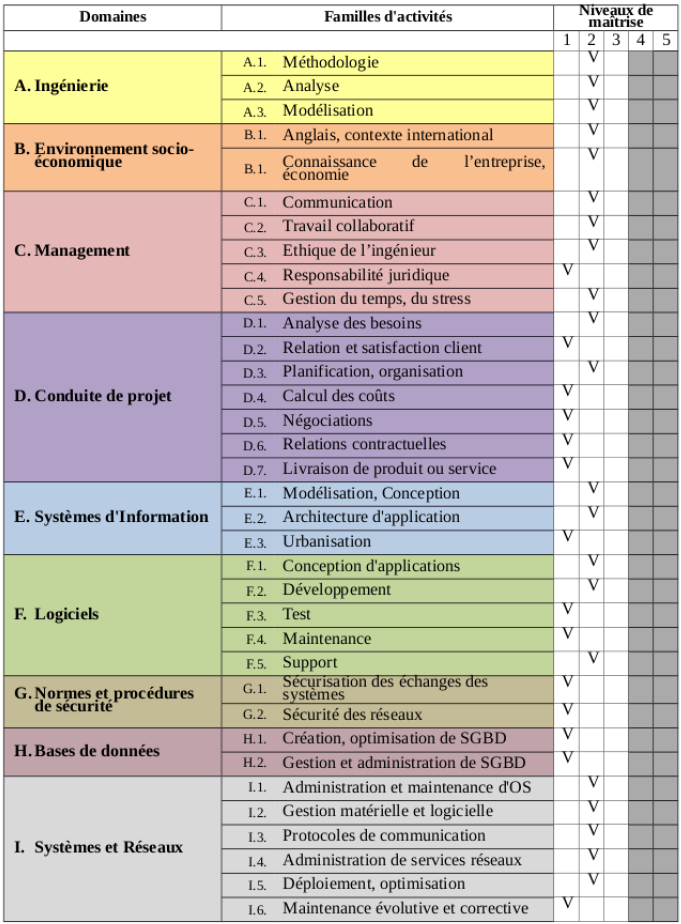
\includegraphics[scale=0.9]{./img/tableaux_cpt.PNG}
    \caption{Tableau d'auto-évaluation des compétences}
\end{figure}

\end{appendix}

\newpage
\printnoidxglossary[type=main]

\end{document}
